\section{Problem Definition}
\label{sec:prob}
Sina Weibo is a social network
in which a user can follow some other users (called {\em friends}),
and be followed by some other users (called {\em followers}).
A follower receives messages posted by his or her friends and can
respond by reposting to the messages.
%Weibo data consists of two parts:
%the friend-follower relation graph and the set of all messages posted
%by these users.

We model the Weibo data as a forest $W$ of {\em message propagation trees}.
A propagation tree $T =$ \pair{V}{E}
is akin to a message thread on forums or bulletin
boards.
Each node $m$ in $V$ represents a text message posted on Weibo which
contains 140 Chinese or Latin characters. $m$ is associated with
meta data $\langle u,~ t,~ c,~i \rangle$,
where $u$ is the creator of the message,
$t$ is the time stamp of the message, $c$ is the type of client from which
the message is sent (e.g., web, mobile, etc.), and $i$ is the set of optional
images which are posted along with the text.
The user information $u$ contains additional
attributes of the user such as gender, number of friends and followers,
number of messages posted in the past, last time of post, etc.
The root node of a tree
is called ``original message'', while all the other nodes in the tree are
called ``reposts'', as they are the responses to either the original message
or other reposts. If there is a directed edge from $m_1$ to $m_2$, then
$m_2$ is a response to $m_1$. For example, the following is the initial
part of a thread where $m_1$ is the original message, and
``//@user1'' means a response to user1.
\begin{itemize}
\small
\item[-] $m_1$ (user1): When a rove beetle is on your skin,
don't crush it or your skin will fester.
\item[-] $m_2$ (user2): Really? I never saw it before! //@user1
\item[-] $m_3$ (user3): Thanks for the warning. //@user1
\item[-] $m_4$ (user4): That sounds awful! What is rove beetle? //@user2
\item[-] $m_5$ (user5): It's true. I've been bitten once. //@user2
\end{itemize}
\figref{fig:ptree} illustrates the corresponding propagation tree.

\begin{figure}[th]
\centering
\epsfig{file=ptree_ex1.eps, width=0.5\columnwidth}
\caption{A Partial Propagation Tree}
\label{fig:ptree}
\end{figure}

In this paper, false rumors and normal messages (which are not false rumors) only refer to the
original Weibo messages and not reposts.
An original message is either a false rumor or a normal message.
%Let $R$ represent the set of all rumors and $N$
%the set of all non-rumors,
%then $U = R \cup N$ is the set of all original messages, or set of all
%roots $root(T)$ for all $T$ the forest $W$.
Our problem is, given a message propagation tree 
$T = $\pair{$V$}{$E$} as well
as the meta data associated with $V$, return whether $root(T)$ is
a false rumor or not.

%we formulate the rumor detection problem as a classification problem. To be more specific, the problem is how to build a classifier that could classify Sina Weibo messages into rumors or non-rumors based on some information of the message and its repost message such as the content of message, the user information of message and the post or repost time of message.

%To solve this problem, In this work, we mainly focus on the propagation features to detect rumors. Hence, we assume the messages which need to be classified have been posted for some time and there are some users who have reposted the message. In other words, out aim is to classify the messages that have been posted not to classify a new message that a user wants to post.
